\documentclass[letter, 11pt]{report}

\usepackage{fullpage}
\usepackage[utf8]{inputenc}
\usepackage[T1]{fontenc}
\usepackage[french]{babel} 
\usepackage{graphicx}
%\usepackage{url} %pour écrire des adresses cliquables
\usepackage{lmodern} %pour changer le pack de police
%\usepackage[top=5cm, bottom=5cm, left=6cm, right=3cm]{geometry} %pour les marges
\usepackage[usenames, dvipsnames]{color}
\usepackage{listings}
\usepackage{hyperref} %pour un fichier PDF  interactif
\usepackage[final]{pdfpages}
\usepackage[table]{xcolor}

\pdfcompresslevel=9

\hypersetup{
	backref=true, %permet d'ajouter des liens dans...
	pagebackref=true, %...les bibliographies
	hyperindex=true, %ajoute des liens dans les index.
	colorlinks=true, %colorise les liens
	breaklinks=true, %permet le retour à la ligne dans les liens trop longs
	urlcolor=blue, %couleur des hyperliens
	linkcolor=blue, %couleur des liens internes
	bookmarks=true, %créé des signets pour Acrobat
	bookmarksopen=true,%si les signets Acrobat sont créés,
	%les afficher complètement.
	%pdftitle={Mon fabuleux livre}, %informations apparaissant dans
	%pdfauthor={Pejvan BEIGUI},%dans les informations du document
	%pdfsubject={Mac OS X}%sous Acrobat.
}


\lstdefinestyle{php}{
	language=PHP,
	caption={PHP},
	basicstyle= \footnotesize,
	tabsize=4,
	showspaces=false,
	showstringspaces=false,
	showtabs=false,
	breaklines=true,
	breakautoindent=true,
	identifierstyle=\color{RoyalBlue},
	commentstyle=\color{LimeGreen},
	keywordstyle=\color{Black},
	stringstyle=\color{OrangeRed},
	backgroundcolor=\color{white},
	numbers=left
}

\begin{document}

\title{Carcajou}
\author{\textsc{Martin Desharnais} \\ \textsc{Samuel Milette-Lacombe} \\ \textsc{Marc-André Destrempes}}
\date{\today}

\maketitle

\begin{abstract}
Ce document contient la documentation du projet de médiathèque (nom de code «~Carcajou~») conçu pour le département de musique du cégep de Trois-Rivières.
\end{abstract}

\newpage
\tableofcontents
\newpage

%%%%%%%%%%%%%%%%%%%%%%%%%%%%%%%%%%%%%%%%%%%%%%%%%%
\chapter{Spécifications fonctionnelles}
%%%%%%%%%%%%%%%%%%%%%%%%%%%%%%%%%%%%%%%%%%%%%%%%%%

\section{Caractéristiques}

\subsection{Fonctions du système}

Les fonctions offertes par notre système de médiathèque sont les suivantes:

Système de recherche et de parcours des médias
\begin{itemize}
	\item Recherche simple de médias
	\item Recherche avancée de médias
	\item Fil d'Ariane vertical permettant de naviguer parmi les médias
	\item Système de pagination avancée permettant de naviguer dans les résultats
\end{itemize}

\subsection{Recherche avancée}

Dans la recherche avancée, lors de la sélection d'un critère d'un recherche, une liste de suggestions est automatiquement liée au champ texte. Dès que l'on tape la première lettre du mot clés, une liste de valeurs ayant cette lettre s'affichera. Cette ajout rend la recherche avancée beaucoup plus conviviale. Cette fonctionnalité utilise la balise « DATALIST » qui disponible uniquement sur des navigateurs supportant cette balise Html 5.

Dans la recherche avancée, il est aussi possible d'ajouter autant de critères de recherches que l'on désire. Pour cela, le javascript a été utilisé pour interragir dinanymiquement avec le DOM de la page. Des effets visuels de disparation et d'apparition ont même été ajouté pour une ergonomie plus dynamique.

\subsection{Médias}
Le client nous a expliquer que certains médias ne peuvent être empruntés que par certains groupes d'utilisateurs alors que d'autres sont disponnibles uniquements pour consultation sur place.

Pour représenter cette situation, nous avons décidés que chaque média contiendra la liste des groupes habilités à l'emprunter. Si aucun groupe n'est défini, cela signifie que personne ne peut l'emprunter et qu'il est disponnible en consultation sur place seulement.

%%%%%%%%%%%%%%%%%%%%%%%%%%%%%%%%%%%%%%%%%%%%%%%%%%
\chapter{Architecture du système}
%%%%%%%%%%%%%%%%%%%%%%%%%%%%%%%%%%%%%%%%%%%%%%%%%%

\section{Charte graphique}

\subsection{Introduction}

Le site internet se veut d'abord sobre et pratique.

\subsection{Maquette}

Toutes les pages sont construites sur la base du modèle suivant :
\newline
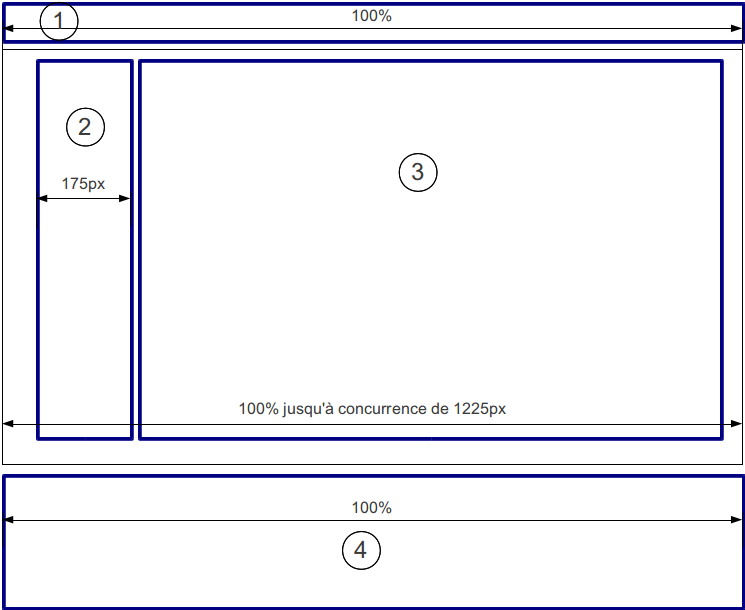
\includegraphics[scale=0.6]{maquetteImage.png}
\newline
1 : Bandeau\newline
2: Fil d'Ariane verticale (n'apparait cependant que dans l'affichage des résultats de recherche)\newline
3: Contenu de la page\newline
4: Pied de page\newline
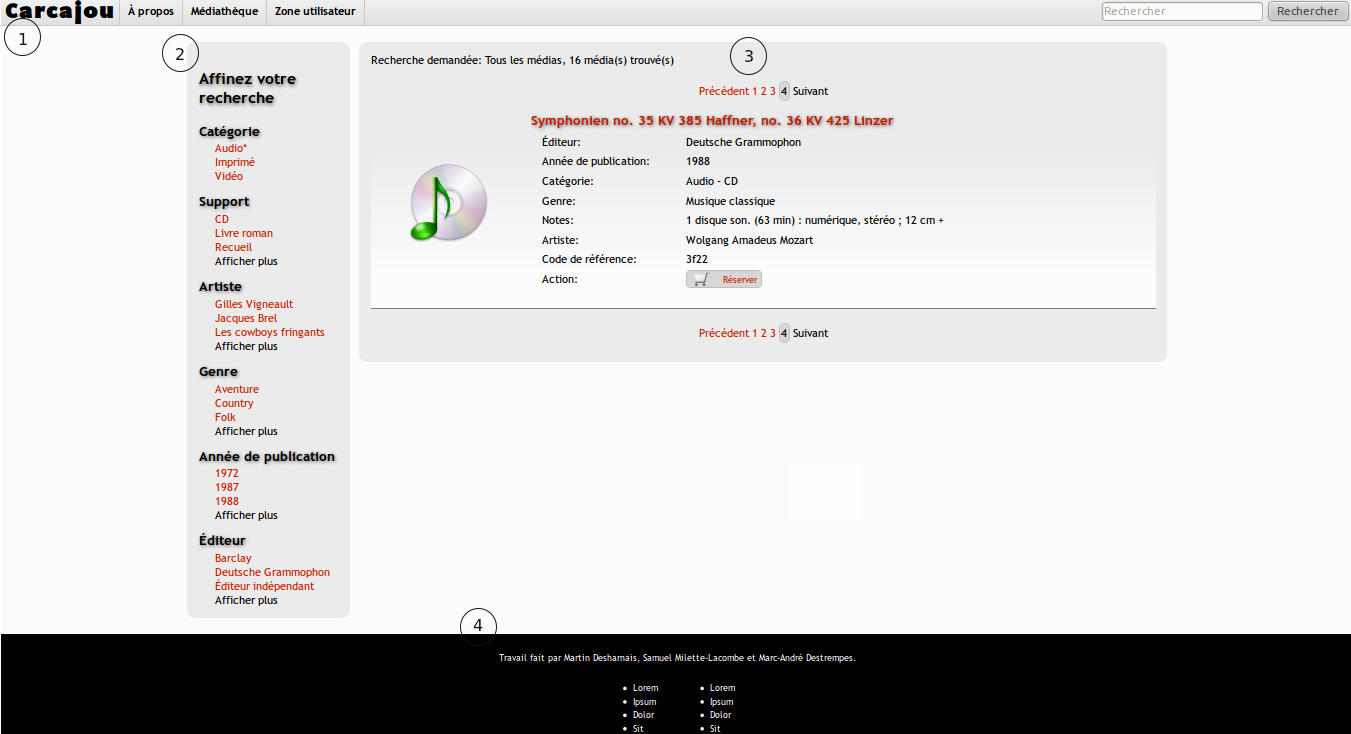
\includegraphics[scale=0.3]{pageType.png}

\subsubsection{Bandeau (1)}

Le bandeau est constitué des éléments suivant:
\begin{description}
	\item[Sigle Carcajou] Le sigle Carcajou est en fait le logo du site. Par contre, ce n'est pas une image mais bien un mot mise en forme en css. Ce sigle permet de revenir sur la page d'accueil (en haut à gauche). Le sigle du site utilise la police MegalopolisExtra-Webfont.
	\item[Menus déroulants]À la droite du sigle se retrouve le menu principal incluant des menus déroulants permettant de se déplacer dans les sections du site. Les entrées de menu sont les suivantes:
		\begin{itemize}
			\item À propos
				\begin{itemize}
					\item De la médiathèque
					\item Du département de musique
					\item Des heures d'ouverture
					\item De la règlementation					
				\end{itemize}
		\end{itemize}
		\begin{itemize}
			\item Médiathèque
			\begin{itemize}
				\item Recherche avancée
				\item Parcourir
				\item Suggestions				
			\end{itemize}
		\end{itemize}
		\begin{itemize}
			\item Zone utilisateur (lorsque non connecté)
			\begin{itemize}
				\item Connexion
				\item Inscription			
			\end{itemize}
		\end{itemize}
		\begin{itemize}
			\item Zone utilisateur (lorsque connecté)
			\begin{itemize}
				\item Mes réservations
				\item Mes emprunts en cours
				\item Mon historique d'emprunts
				\item Déconnexion
			\end{itemize}
		\end{itemize}
			\begin{itemize}
			\item Administration (lorsque connecté)
			\begin{itemize}
				\item Emprunt
				\item Retour
				\item Générer code QR
			\end{itemize}
		\end{itemize}
	\item[Champ de recherche simple] Le champ texte accompagné du bouton «~Rechercher~» permet d'effectuer une recherche simple avec un mot clé.
\end{description}

\subsubsection{Fil d'Ariane vertical (2)}
Le fil d'Ariane vertical permet d'afficher des critères permettant d'avatange la recherche. Il contient des éléments liste contenant des liens pour raffiner la recherche.

\subsubsection{Contenu (3)}
Le contenu des pages est affiché dans cette partie. Son contenu varie énormément selon la page affichée. Dans la capture d'écran présente ci-haut, on y voit les résultats d'une recherche.

\subsubsection{Pied de page (4)}
Les noms des auteurs sont affichés dans cette partie. Le pied de page contient aussi, sous forme de listes, des liens vers différentes sections du site comme on le voit si souvent dans les tendances actuelles du web. Le principe d'afficher plusieurs liens divers dans le pied de page offre la possibilité d'offrir une navigation alternative au menu conventionnel. À la phase conception, le pied ne contient pas encore de véritables liens. Seuls des liens d'exemple «~Lorem Ipsum~» sont affichés.

\subsection{Charte graphique}


\subsubsection{Couleurs}

\begin{table}[h]
	\caption{couleurs}
	\begin{center}
		\begin{tabular}{|l|l|l|}
		\hline
		Element    					& Code     & Apercu \\ \hline
		\multicolumn{3}{|c|}{Header} \\ \hline
		background 					& \#000000 & \cellcolor[HTML]{000000} \\ \hline
		h1         					& \#FFFFFF & \cellcolor[HTML]{FFFFFF} \\ \hline
		nav        					& \#FFFFFF & \cellcolor[HTML]{FFFFFF} \\ \hline
		ul         					& \#FFFFFF & \cellcolor[HTML]{FFFFFF} \\ \hline
		li         					& \#FFFFFF & \cellcolor[HTML]{FFFFFF} \\ \hline
		a          					& \#FFFFFF & \cellcolor[HTML]{FFFFFF} \\ \hline
		h1:hover   					& \#FFFFFF & \cellcolor[HTML]{FFFFFF} \\ \hline
		nav:hover  					& \#FFFFFF & \cellcolor[HTML]{FFFFFF} \\ \hline
		ul:hover   					& \#FFFFFF & \cellcolor[HTML]{FFFFFF} \\ \hline
		li:hover   					& \#FFFFFF & \cellcolor[HTML]{FFFFFF} \\ \hline
		a:hover    					& \#FFFFFF & \cellcolor[HTML]{FFFFFF} \\ \hline
		h1:focus   					& \#FFFFFF & \cellcolor[HTML]{FFFFFF} \\ \hline
		nav:focus  					& \#FFFFFF & \cellcolor[HTML]{FFFFFF} \\ \hline
		ul:focus   					& \#FFFFFF & \cellcolor[HTML]{FFFFFF} \\ \hline
		li:focus   					& \#FFFFFF & \cellcolor[HTML]{FFFFFF} \\ \hline
		a:focus    					& \#FFFFFF & \cellcolor[HTML]{FFFFFF} \\ \hline
		\multicolumn{3}{|c|}{Footer} \\ \hline
		background 					& \#000000 & \cellcolor[HTML]{000000} \\ \hline
		nav        					& \#FFFFFF & \cellcolor[HTML]{FFFFFF} \\ \hline
		ul         					& \#FFFFFF & \cellcolor[HTML]{FFFFFF} \\ \hline
		li         					& \#FFFFFF & \cellcolor[HTML]{FFFFFF} \\ \hline
		a          					& \#FFFFFF & \cellcolor[HTML]{FFFFFF} \\ \hline
		\multicolumn{3}{|c|}{Content} \\ \hline
		background 					& \#FFFFFF & \cellcolor[HTML]{FFFFFF} \\ \hline
		a							& \#C52100 & \cellcolor[HTML]{C52100} \\ \hline
		\multicolumn{3}{|l|}{Pagination} \\ \hline
		background 					& \#DBD9D9 & \cellcolor[HTML]{DBD9D9} \\ \hline
		border 	   					& \#C1C1C1 & \cellcolor[HTML]{C1C1C1} \\ \hline
		\multicolumn{3}{|l|}{Résultat recherche} \\ \hline
		a:background 				& \#DBD9D9 & \cellcolor[HTML]{DBD9D9} \\ \hline
		a:border   					& \#C1C1C1 & \cellcolor[HTML]{C1C1C1} \\ \hline
		tr:border  					& \#C0C0C0 & \cellcolor[HTML]{C0C0C0} \\ \hline
		\multicolumn{3}{|l|}{Médias} \\ \hline
		textarea:border 			& \#C0C0C0 & \cellcolor[HTML]{C0C0C0} \\ \hline
		\multicolumn{3}{|l|}{Style} \\ \hline
		background 					& \#E3E3E3 & \cellcolor[HTML]{E3E3E3} \\ \hline
		h1 							& \#FFFFFF & \cellcolor[HTML]{FFFFFF} \\ \hline
		a:focus 					& \#FFFFFF & \cellcolor[HTML]{FFFFFF} \\ \hline
		nav > ul a:focus 			& \#EEEEEE & \cellcolor[HTML]{EEEEEE} \\ \hline
		nav > ul a:hover 			& \#EEEEEE & \cellcolor[HTML]{EEEEEE} \\ \hline
		nav > ul > li 				& \#CCCCCC & \cellcolor[HTML]{CCCCCC} \\ \hline
		nav > ul > li:first-child 	& \#CCCCCC & \cellcolor[HTML]{CCCCCC} \\ \hline
		nav > ul > li ul:border-top & \#CCCCCC & \cellcolor[HTML]{CCCCCC} \\ \hline
		nav > ul > li ul:border 	& \#EEEEEE & \cellcolor[HTML]{EEEEEE} \\ \hline
		\end{tabular}
	\end{center}
\end{table}

\subsection{Typographie}

\subsubsection{Police d’écriture}

La police de caractère du site est Optima, Trebuchet MS, Lucida, Arial, Geneva, Verdana, Lucida Grande, Tahoma, Helvetica, sans-serif. Elle aura une grosseur de 1em.

\subsubsection{Titres}
Les titres sont de la même police de caractère que le reste du site. 

\begin{table}
	\caption{Taille des polices}
	\begin{center}
		\begin{tabular}{|c|c|}
			\hline
			Titre & Taille \\
			\hline
			h1  & 1.9em\\
			h2  & 1.75em\\
			h3  & 1.4em\\
			h4  & 1.2em\\
			h5  & 1.15em\\
			h5  & 1.1em\\
			\hline
		\end{tabular}
	\end{center}
\end{table}

\subsubsection{Majuscules-minuscules}

Tous les titres commencent par une majuscule suivis par des minuscules. Il en est de même pour tout le texte contenu dans la page, c'est à dire, les paragraphes, les liens, etc.

\subsubsection{Arborescense du site}

A generer a l'aide de visio ou a la main

\subsubsection{Images}

\begin{table}[ht]
	\caption{images}
	\begin{center}
		\begin{tabular}{|c|l|p{5cm}|}
		\hline
		Image 		& Taille 			& Description \\ \hline
		
\includegraphics[scale=0.2]{black_arrow_big.png} 	& 370x216, 209x122 	& Cette image servira a afficher les détails d'un média. \\ \hline
		
\includegraphics{cart.png} 							& 20x20 			& Panier signifiant la réservation d'un média. \\ \hline
		
\includegraphics[scale=1.15]{emprunt.png} 			& 87x87 			& Logo signifiant un emprunt. \\ \hline
		
\includegraphics[scale=0.3]{reservation.png} 		& 87x87 			& Logo signifiant une réservation. \\ \hline
		
\includegraphics[scale=0.3]{musique.png} 			& 128x105 			& Logo signifiant de la musique. \\ \hline
		
\includegraphics[scale=0.3]{audio.png} 				& 128x128 			& Logo signifiant la présence d'un média sous le format audio. \\ \hline
		
\includegraphics[scale=0.3]{imprime.png} 			& 128x128 			& Logo signifiant la présence d'un média sous le format imprimé. \\ \hline
		
\includegraphics[scale=0.3]{video.png} 				& 128x128 			& Logo signifiant la présence d'un média sous le format vidéo. \\ \hline
		
\includegraphics[scale=0.3]{search.png} 			& 128x128, 32x32 	& Icone signifiant l'exécution d'une recherche. \\ \hline
		
\includegraphics{down.png} 							& 21x4 				& Flèche pointant vers le haut. \\ \hline
		
\includegraphics{up.png} 							& 21x4 				& Flèche pointant vers le bas. \\ \hline
		
\includegraphics{upAndDown.png} 					& 21x9 				& Flèches pointant vers le haut et vers le bas. \\ \hline
		
\includegraphics{img_puce_search.png} 				& 8x12 				& Flèche pointant vers la droite. \\ \hline
		\end{tabular}
	\end{center}
\end{table}

\section{Modèle des pages principales et secondaires}


\section{Diagramme d'enchaînement}
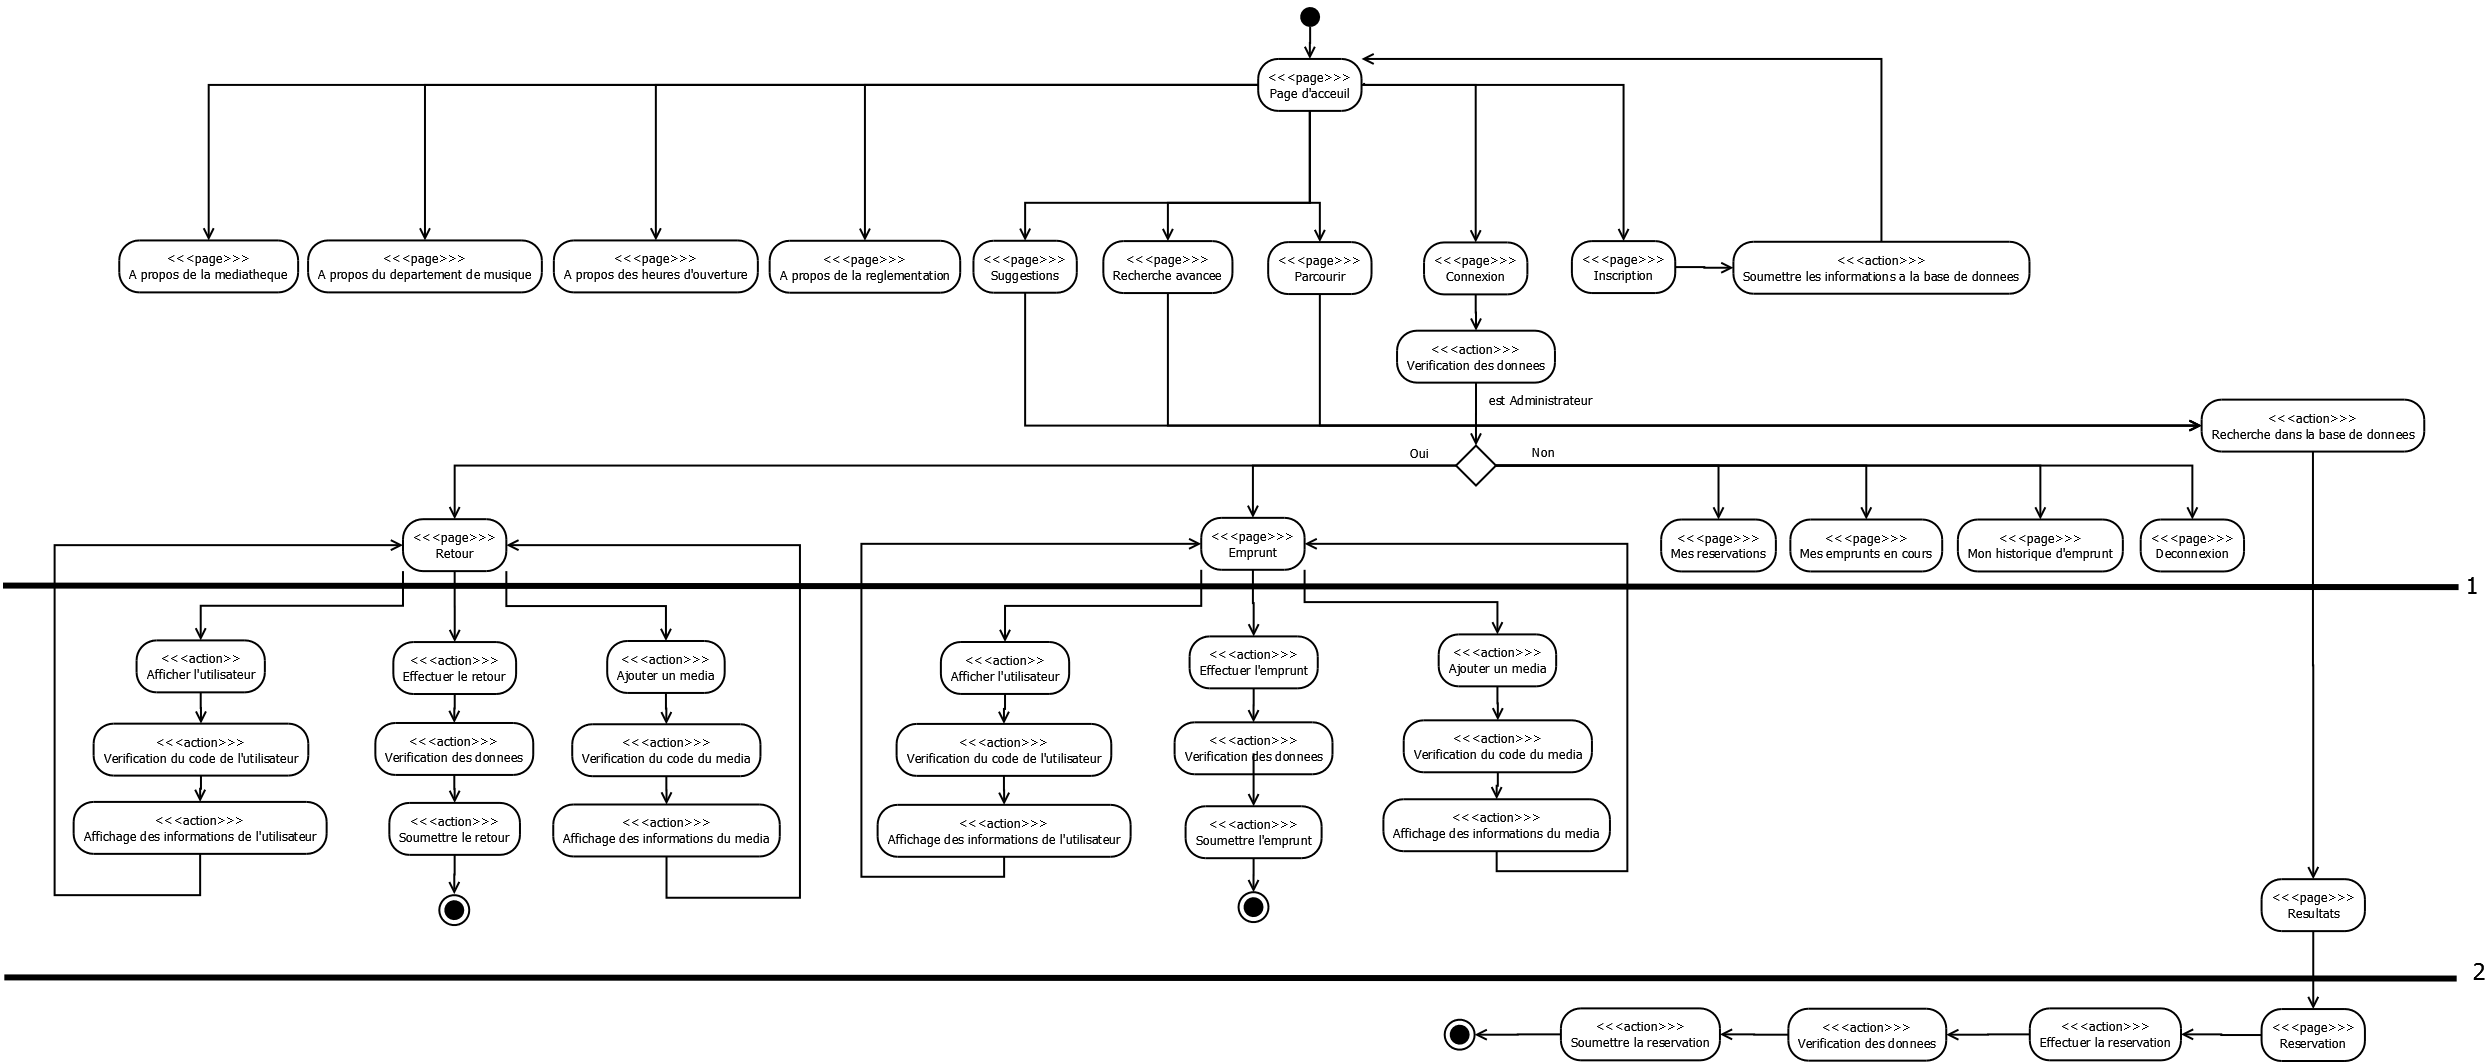
\includegraphics[scale=0.145]{diagrammeEnchainement.png}

Pour accéder au niveau 2 du diagramme, nous devons emprunter exactement le chemin indiqué dans le schéma. Le niveau inférieur peut, en tout temps, accéder aux pages du niveau supérieur.
Lors d'une connexion, si l'utilisateur n'est pas un administrateur nous ne lui affichons pas les pages emprunt et retour. Sinon, nous lui rajoutons ces options dans le menu.

\section{Diagramme de classe}

Voir l'API du système fournis avec le document.

\section{Base de données et dictionnaire}

Voir le tableau en annexe.

%%%%%%%%%%%%%%%%%%%%%%%%%%%%%%%%%%%%%%%%%%%%%%%%%%
\chapter{Architecture technologique}
%%%%%%%%%%%%%%%%%%%%%%%%%%%%%%%%%%%%%%%%%%%%%%%%%%

\section{Représentation graphique}
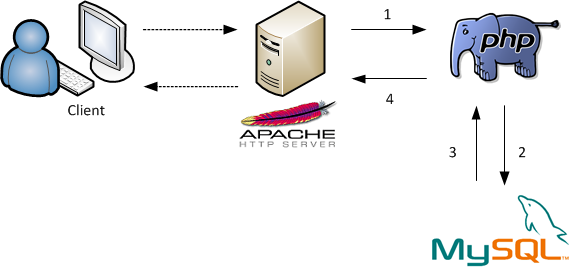
\includegraphics[scale=0.7]{architectureTechnologique.png}

\section{Spécifications techniques}


\subsection{Navigateurs}
Lors de la conception le site à été testé sur les navigateurs suivants~:

\begin{itemize}
	\item Mozilla Firefox 3.5.16
	\item Mozilla Firefox 3.6.10
	\item Mozilla Firefox 4.0.1
	\item Google Chrome 6.0.472.63
	\item Google Chrome 11.0.696.65
\end{itemize}

Le site est fonctionnel sur l'ensemble des navigateurs mais certains effets graphiques ne sont disponnibles que sur les versions récentes de chacun.

\subsection{Languages}
\subsubsection{Client}
Du coté client, les languages utilisés sont le HTML 5, le CSS 3, le javascript et le XML.

Pour le HTML 5 et le CSS 3, il a été décidé d'utiliser les fonctionnalitées dont nous avions besoin tout en gardant en tête que le site devait rester consultable sur les navigateurs ne reconnaissant pas ces nouvelles technologies. Par exemple, la propriété CSS 3 «~border-radius~» nous permet d'afficher des coins arrondis facilement sur n'importe quel composant de la page. Dans le cas où celle-ci ne serait pas reconnue par un navigateur, celui-ci doit ignorera simplement la propriété et affichera des coins carrés standards.

Pour le javascript, la bibliothèque \href{http://jquery.com/}{jQuery 1.6.1} a été utiliser afin de simplifier le code et d'unifier la gestion des différents navigateurs. En effet cette bibliothèque a l'avantage de proposer des fonctions unifiées qui se chargent pour nous de gérer les différences entre les différents navigateurs.

Cependant, il a été décidé de réduire au maximum la dépendance au javascript. Dans le cas de fonctionnalités javascript facultatives, comme le fait de n'afficher que les trois premier éléments des listes trop longues, le code HTML ne contient qu'une liste toute simple et c'est au chargement de la page par le navigateur que le javascript s'occupe de modifier la structure du document et d'offire un bouton permettant d'afficher les éléments excédentaires.

Bien sur, il y certains cas où le javascript est absolument obligatoire, comme la création de nouveau champs dans les formulaires devant traiter un nombre variables d'enregistrements. Heureusement, ces cas complexes ne s'appliquent que dans des sections d'administration. Un visiteur ou un utilisateur disposant de droits minimaux peut donc se passer aisément de javascript et le site reste parfaitement consultable.

Pour le XML, celui-ci est utilisé comme moyen de transmission de l'information lors des requêtes AJAX. À l'heure actuelle, les requêtes AJAX sont faites à des fichers XML statiques mais, à terme, des scripts PHP devrons être écrits permettant de générer dynamiquement le fichier selon les critères reçus en paramètre.

\subsubsection{Serveur}
Du coté serveur, le seul language utilisé est le PHP, qui a été utilisé dans ses versions 5.3.3 et 5.3.5 dépendamment des contributeurs.

Les conventions php utilisés sont les suivantes~:

\begin{itemize}
	\item Les fichiers contenant la définition d'une classe PHP utilisent l'extension «~.class.php~».
	\item Les fichiers contenant du code PHP qui ne fait rien par lui-même et doit obligatoirement être inclu par un autre script utilisent l'extension «~.inc.php~».
	\item Les fichiers contenant du code PHP qui se suffit à lui-même utilisent l'extension «~.php~».
	\item Les fichiers contenant les pages finales affichées à l'utilisateur sont situés à la racine du projet (/).
	\item Les fichiers contenant des scripts PHP qui effectuent une action avant de rediriger l'utilisateur sont situés dans le répertoire php (/php/).
\end{itemize}

\subsection{Bande passante}
L'utilisation et l'administration du site nécessitent une bande passante standard.

\subsection{Serveurs}
Apache HTTP Server 2.2.16 -- 2.2.17

\subsection{Type de base de données}
MySQL 5.1.49 -- 5.5.8

\section{Sécurité}
\subsection{En théorie}

La gestion des droits fait appel au «~bit~bashing~», une technique qui consiste à donner une représentation binaire à chacun des droits et de ne stocker que la somme de ces droits dans la base de données. Ainsi, si nous avons les droits suivants de définis~:

\begin{itemize}
	\item \$application->rights['read'] = 0001
	\item \$application->rights['write'] = 0010
	\item \$application->rights['execute'] = 0100
\end{itemize}

et qu'un groupe A dispose des droits de lecture et d'écriture dans la section «~administration~», et qu'un groupe B dispose du droit de renouveler un prêt la table droits\_groupes contiendrait quelque chose comme ceci~:

\begin{table}[ht]
	\caption{groupes}
	\begin{center}
		\begin{tabular}{|c|l|l|}
			\hline
			ID & nom & inactif \\
			\hline
			1  & A   & FALSE \\
			2  & B   & FALSE \\
			\hline
		\end{tabular}
	\end{center}
\end{table}

\begin{table}[h!]
	\caption{droits\_groupes}
	\begin{center}
		\begin{tabular}{|c|l|c|l|}
			\hline
			ID & section                 & groupeID & droits \\
			\hline
			1  & administration          & 1        & 0011 \\
			2  & Renouveller un document & 1        & 0100 \\
			3  & Renouveller un document & 2        & 0100 \\
			\hline
		\end{tabular}
	\end{center}
\end{table}

Dans cet exemple, nous pouvons voir que le groupe A dispose des droits de lecture et d'écriture ($ 0001 + 0010 = 0011 $) sur la section «~administration~» et qu'il a le droit de renouveler des documents puisqu'il a le droit d'exécution (0100) sur «~extendLoan~».

Le groupe B, tant qu'à lui, ne dispose que du droit de renouveler des documents. En effet, si aucune entrée ne correspond à un groupe pour une section données, il est assumé que ledit groupe n'a aucun droit sur cette section. Le fait de ne créer aucun enregistrement est strictement équivalent au fait de créer un enregistrement contenant les droits (0000).

\begin{table}[h!]
	\caption{utilisateurs}
	\begin{center}
		\begin{tabular}{|c|l|l|l|l|}
			\hline
			ID & matricule & nom         & prenom   & inactif \\
			\hline
			1  & 11111111  & Baggins     & Frodo    & FALSE \\
			2  & 22222222  & Gamgee      & Samwise  & FALSE \\
			3  & 33333333  & Brandybuck  & Meriadoc & TRUE \\
			4  & 44444444  & Took        & Peregrin & FALSE \\
			\hline
		\end{tabular}
	\end{center}
\end{table}

\begin{table}[h!]
	\caption{groupes}
	\begin{center}
		\begin{tabular}{|c|l|l|}
			\hline
			ID & nom               & inactif \\
			\hline
			1  & Administrateurs   & FALSE \\
			2  & Enseignants       & FALSE \\
			3  & Commis            & FALSE \\
			4  & Étudiants         & FALSE \\
			5  & Prêtre            & TRUE \\
			\hline
		\end{tabular}
	\end{center}
\end{table}

\begin{table}[h!]
	\caption{groupes\_utilisateurs}
	\begin{center}
		\begin{tabular}{|c|c|c|}
			\hline
			ID & exID & groupeID \\
			\hline
			1  & 1    & 1 \\
			2  & 2    & 4 \\
			3  & 2    & 3 \\
			4  & 3    & 4 \\
			5  & 4    & 2 \\
			\hline
		\end{tabular}
	\end{center}
\end{table}

\begin{table}[h!]
	\caption{droits\_groupes}
	\begin{center}
		\begin{tabular}{|c|l|c|c|}
			\hline
			ID & section                & groupeID & droits \\
			\hline
			1  & drivingTable.php       & 1        & 0011 \\
			2  & drivingTable.php       & 2        & 0001 \\
			3  & drivingTable.php       & 3        & 0001 \\
			4  & drivingTable.php       & 5        & 0001 \\
			5  & Renouveler un document & 1        & 0100 \\
			6  & Renouveler un document & 2        & 0100 \\
			7  & Renouveler un document & 3        & 0100 \\
			8  & Renouveler un document & 4        & 0100 \\
			9  & Renouveler un document & 5        & 0100 \\
			10 & Emprunter un document  & 1        & 0100 \\
			11 & Emprunter un document  & 2        & 0100 \\
			12 & Emprunter un document  & 3        & 0100 \\
			13 & Emprunter un document  & 5        & 0100 \\
			\hline
		\end{tabular}
	\end{center}
\end{table}

L'exemple précédant couvre la plupart des situations qui peuvent survenir.

La table «~utilisateurs~» nous informe qu'il y a quatre utilisateurs d'enregistrés dans le système mais que l'un d'entre eux est inactif. Un utilisateur inactif pert automatiquement tous ses droits.

La table «~groupes~» nous informe qu'il y a cinq groupes d'enregistrés dans le système mais que l'un d'entre eux est inactif. Un groupe inactif pert automatiquement tous ses droits et ne peut plus être assigné à de nouveaux utilisateurs.

La table «~groupes\_utilisateurs~» nous informe que l'utilisateur 1 (Frodo Baggins) fait partit du groupe \emph{Administrateurs}\footnote{Par convention, le groupe \emph{Administrateurs} dispose généralement de tous les droits sur le système.}, que l'utilisateur 2 (Samwise Gamgee) fait partit à la fois du groupe \emph{Étudiants} et du groupe \emph{Commis}, que l'utilisateur 3 (Meriadoc Brandybuck) fait partit du groupe \emph{Étudiants} et, finalement, que l'utilisateur 4 (Peregrin Took) fait partit du groupe \emph{Enseignants}.

Enfin, la table «~droits\_groupes~» nous informe si chaque groupe peut~:

\begin{itemize}
	\item Afficher et/ou modifier les résulats de la page drivingTable.php;
	\item Effectuer l'action de renouveler un document;
	\item Effectuer l'action d'emprunter un document.
\end{itemize}

Nous voyons ainsi que les commis et les enseignants ont accès à la page drivingTable.php en lecture seule et que les administrateurs y ont accès en lecture-écriture. Les prêtres auraient aussi eu accès en lecture seule, mais en désignant leur groupe comme inactif, ils ont perdu tous leur droits; L'enregistrement numéro 4 doit donc être ignoré par le processur de traitement des droits. Les étudiant, quant à eux, n'ont aucun enregistrement correspondant à cette section. Il est alors assumé qu'ils n'ont aucun droit sur la page drivingTable.php.

Nous voyons que tous les groupes d'utilisateurs ont le droit de renouveller un document mais, encore une fois, l'enregistrement concernant les prêtres doit être ignoré.

Nous voyons enfin que tous les groupes, à l'exception des étudiants, ont le droit d'effectuer un emprunt\footnote{Veuillez noter que c'est le fait d'entrer un nouvel emprunt dans le système qui est traité ici. En effet, un simple étudiant doit demander à un commis qui, lui, se chargera d'entrer sont emprunt dans le système.}.

Les utilisateurs actifs disposent de la somme des droits de chacun de groupes actifs auxquels ils appartiennent. Ainsi, Samwise Gamgee, qui est à la fois un étudiant et un commis, gagne le droit de consulter la page drivingTable.php en lecture seule et d'entrer des emprunts dans le système alors que Perigrin Took, qui est iniactif, n'a aucun droit sur le système, quels que soient les groupes auxquels il appartient.

\subsection{En pratique}
La sécurité repose essentiellement sur la validation des droits des utilisateurs lors de la génération des pages du site. C'est le PHP qui est chargé de valider que l'utilisateur courant dispose des droits suffisants avant d'ajouter une section à la page que le serveur HTTP s’apprête à retourner.

En pratique cela se traduit par un appel à la fonction \$application->currentUser->haveRights() en lui spécifiant en premier paramètre la section dont l'on veut tester les droits et en second paramètre la liste des droits dont l'utilisateur doit disposer pour avoir accès à ce contenu. Ces droits sont définis dans le tableau \$application->rights. Par exemple afin de valider que l'utilisateur a bien le droit d'accéder à la zone d'administration, il suffit d'utiliser le code suivant~:

\begin{lstlisting}[style=php]
if($application->currentUser->haveRights('administration', $application->rights['read'] | $application->rights['write']))
{
	// We can now print administration section
}
else
{
	// Current user does not have suffisent rights
}
\end{lstlisting}

Du point de vu de l'utilisateur de la fonction, c'est extrèmement simple. Pour celui qui devra l'implémanter, c'est une autre histoire. Plaçons-nous un peu à la place du programmeur. Nous sommes dans une fonction dont voici la signature~:

\begin{lstlisting}[style=php]
public function haveRights($section, $rights)
{
	// TODO: Implement function
}
\end{lstlisting}

Pour atteindre son but, il dispose des informations suivantes :

\begin{itemize}
	\item \$section qui est la section dont l'on veut tester les droits;
	\item \$rights qui sont les droits que l'on doit tester;
	\item \$application->currentUser retourne une instance de la classe User représentant l'utilisateur actuellement connecté;
	\item \$application->database retourne une instance de la classe PDO représentant la base de données;
	\item \$application->rights retourne un tableau associatif contenant la représentation numérique de tous droits.
\end{itemize}

Pour pouvoir déterminer si l'utilisateur courrant a bien les droits demandés, il faudra exécuter une requête à la base de données qui nous retourne la liste de tous les droits qu'à cet utilisateur sur cette section\footnote{Il peut y en avoir plus d'un si l'utilisateur appartient à plus d'un groupe.}, additionner ces droits gràce à l'\href{http://www.php.net/manual/en/language.operators.bitwise.php}{opérateur «~ou~binaire~»} (binary or) et déterminer si tous les bits à 1 dans les droits demandés sont aussi à 1 dans les bits des droits de l'utilisateur gràce à l'opérateur «~et~binaire~» (binary and).

\subsection{En conclusion}
Cette façon de gérer les droits des utilisateurs offre de nombreux aventages~:

\begin{itemize}
	\item La plus grande partie de la gestion des droits est centralisée dans la base de données plutôt que de s'éparpiller dans de multiples fichiers;
	\item La notions de groups permet de généraliser des droits semblables à de nombreux utilisateurs;
	\item Le fait qu'un utilisateur puisse appartenir à plusieurs groupes permet un haut niveau de granularité, tout en restant facultatif;
	\item Le fait qu'un groupe ne dispose que des droits explicitement définies assure la sécurité car tous nouveau droit n'est effectif que pour ceux qui l'on explicitement reçus.
	\item L'utilisation du «~bit~bashing~» plutôt que des colonnes explicitement définies permet d'ajouter très façilement de nouveaux types de droits à ceux déjà définis (read, write, execute).
\end{itemize}

%%%%%%%%%%%%%%%%%%%%%%%%%%%%%%%%%%%%%%%%%%%%%%%%%%
\chapter{Prototype fonctionnel}
%%%%%%%%%%%%%%%%%%%%%%%%%%%%%%%%%%%%%%%%%%%%%%%%%%

\appendix

\chapter{Dictionnaire de données}
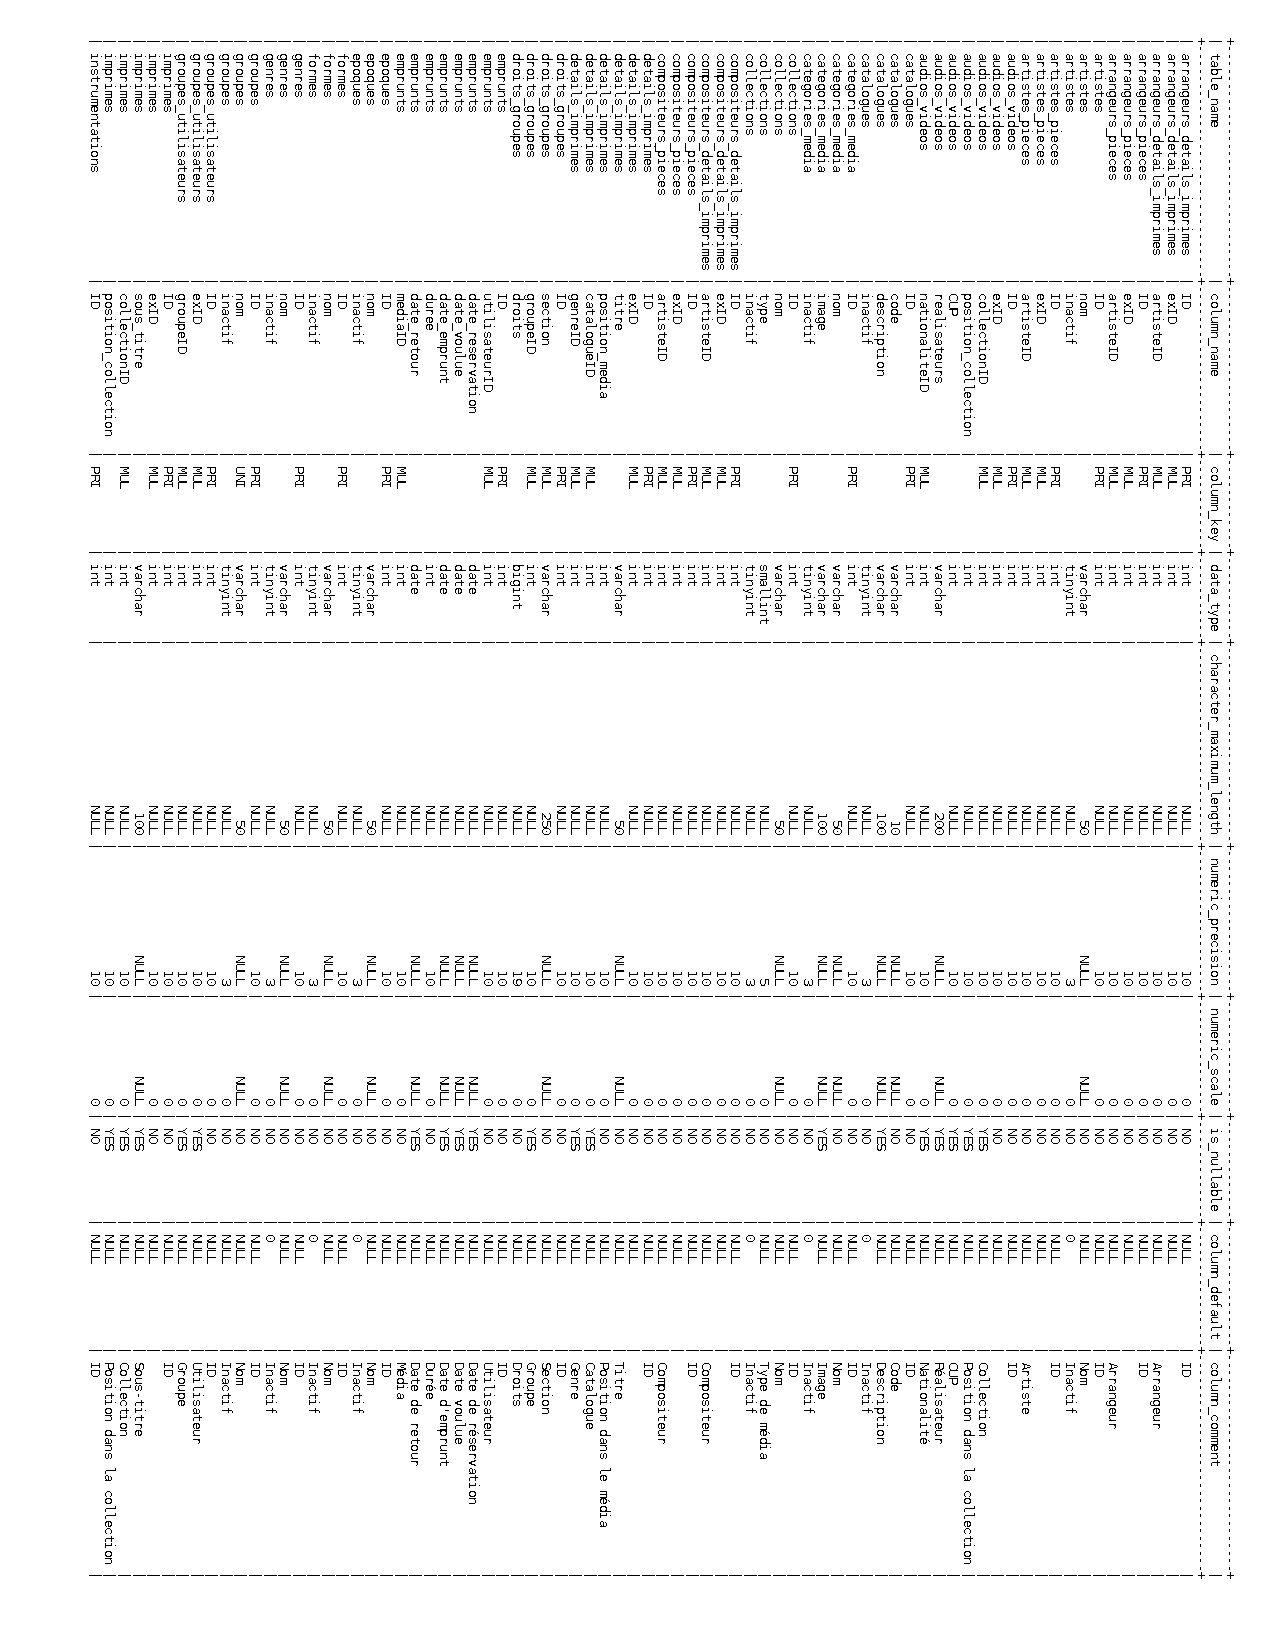
\includepdf[pages=-]{dataDictionary.pdf}

\listoffigures
\listoftables

\end{document}
